\chapter{Instructions for Construction}
\label{chap:construction}

In order to create this product, you should have some level for familiarity
with electronics (i.e., reading a schematic) and be comfortable using a
computer from the command line/terminal. Please purchase all items from the
Bill of Materials (\autoref{chap:bom}). You will also need some assorted 24 AWG
wires, a wire cutter/stripper tool, and a knife.

The following instructions will lead you through the process of building the
\textit{RotaSense} and downloading the necessary code.

\begin{enumerate}
\item Install PlatformIO IDE following their official directions:
  \href{https://platformio.org/platformio-ide}{https://platformio.org/platformio-ide}.
  
\item Cut the sticky tape on the bottom of the breadboard in between the power
  rails and main body.
  \begin{figure}[H]
    \centering
    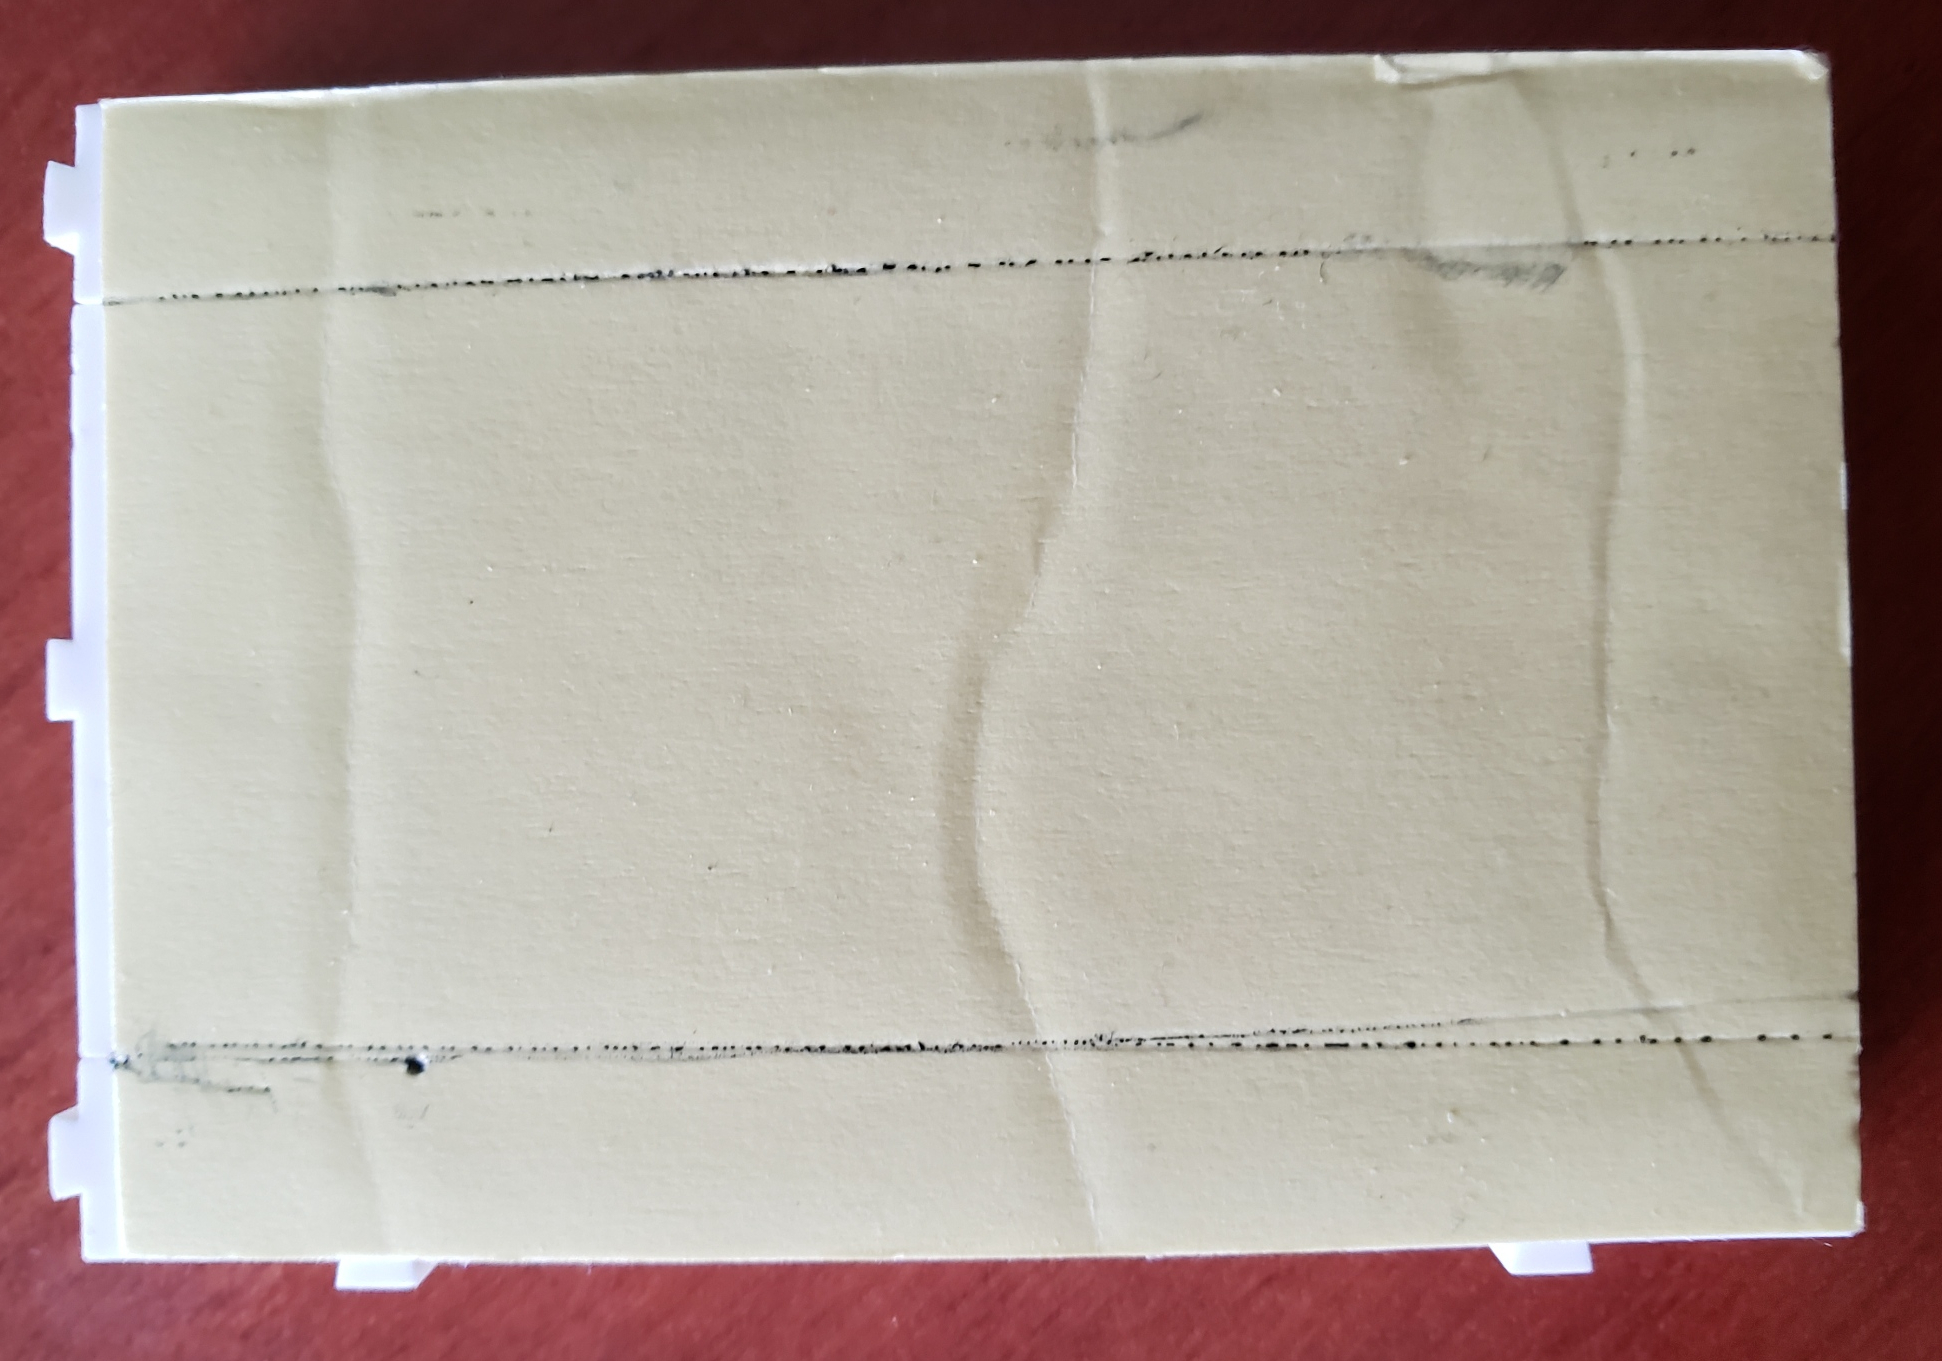
\includegraphics[width=0.5\textwidth]{bb_cuts}
    \caption{Where to cut the sticky tape on the breadboard.}
    \label{fig:bb-cuts}
  \end{figure}
  
\item Slide the power rails off the main breadboard body.\\
  \textit{Hint: one rail slides up, the other down.}
  
\item Insert the ESP32 into the breadboard, with USB port facing outwards, and
  run wires as shown. A detailed schematic can be found in \autoref{fig:schematic}.\\
  \\
  The red wire runs from \textit{A12} to \textit{F8}.\\
  The black wire runs from \textit{J18} to \textit{G7}.\\
  The blue wire runs from \textit{J17} to \textit{J5}.\\
  The green wire runs from \textit{J14} to \textit{J6}.
  \begin{figure}[H]
    \centering
    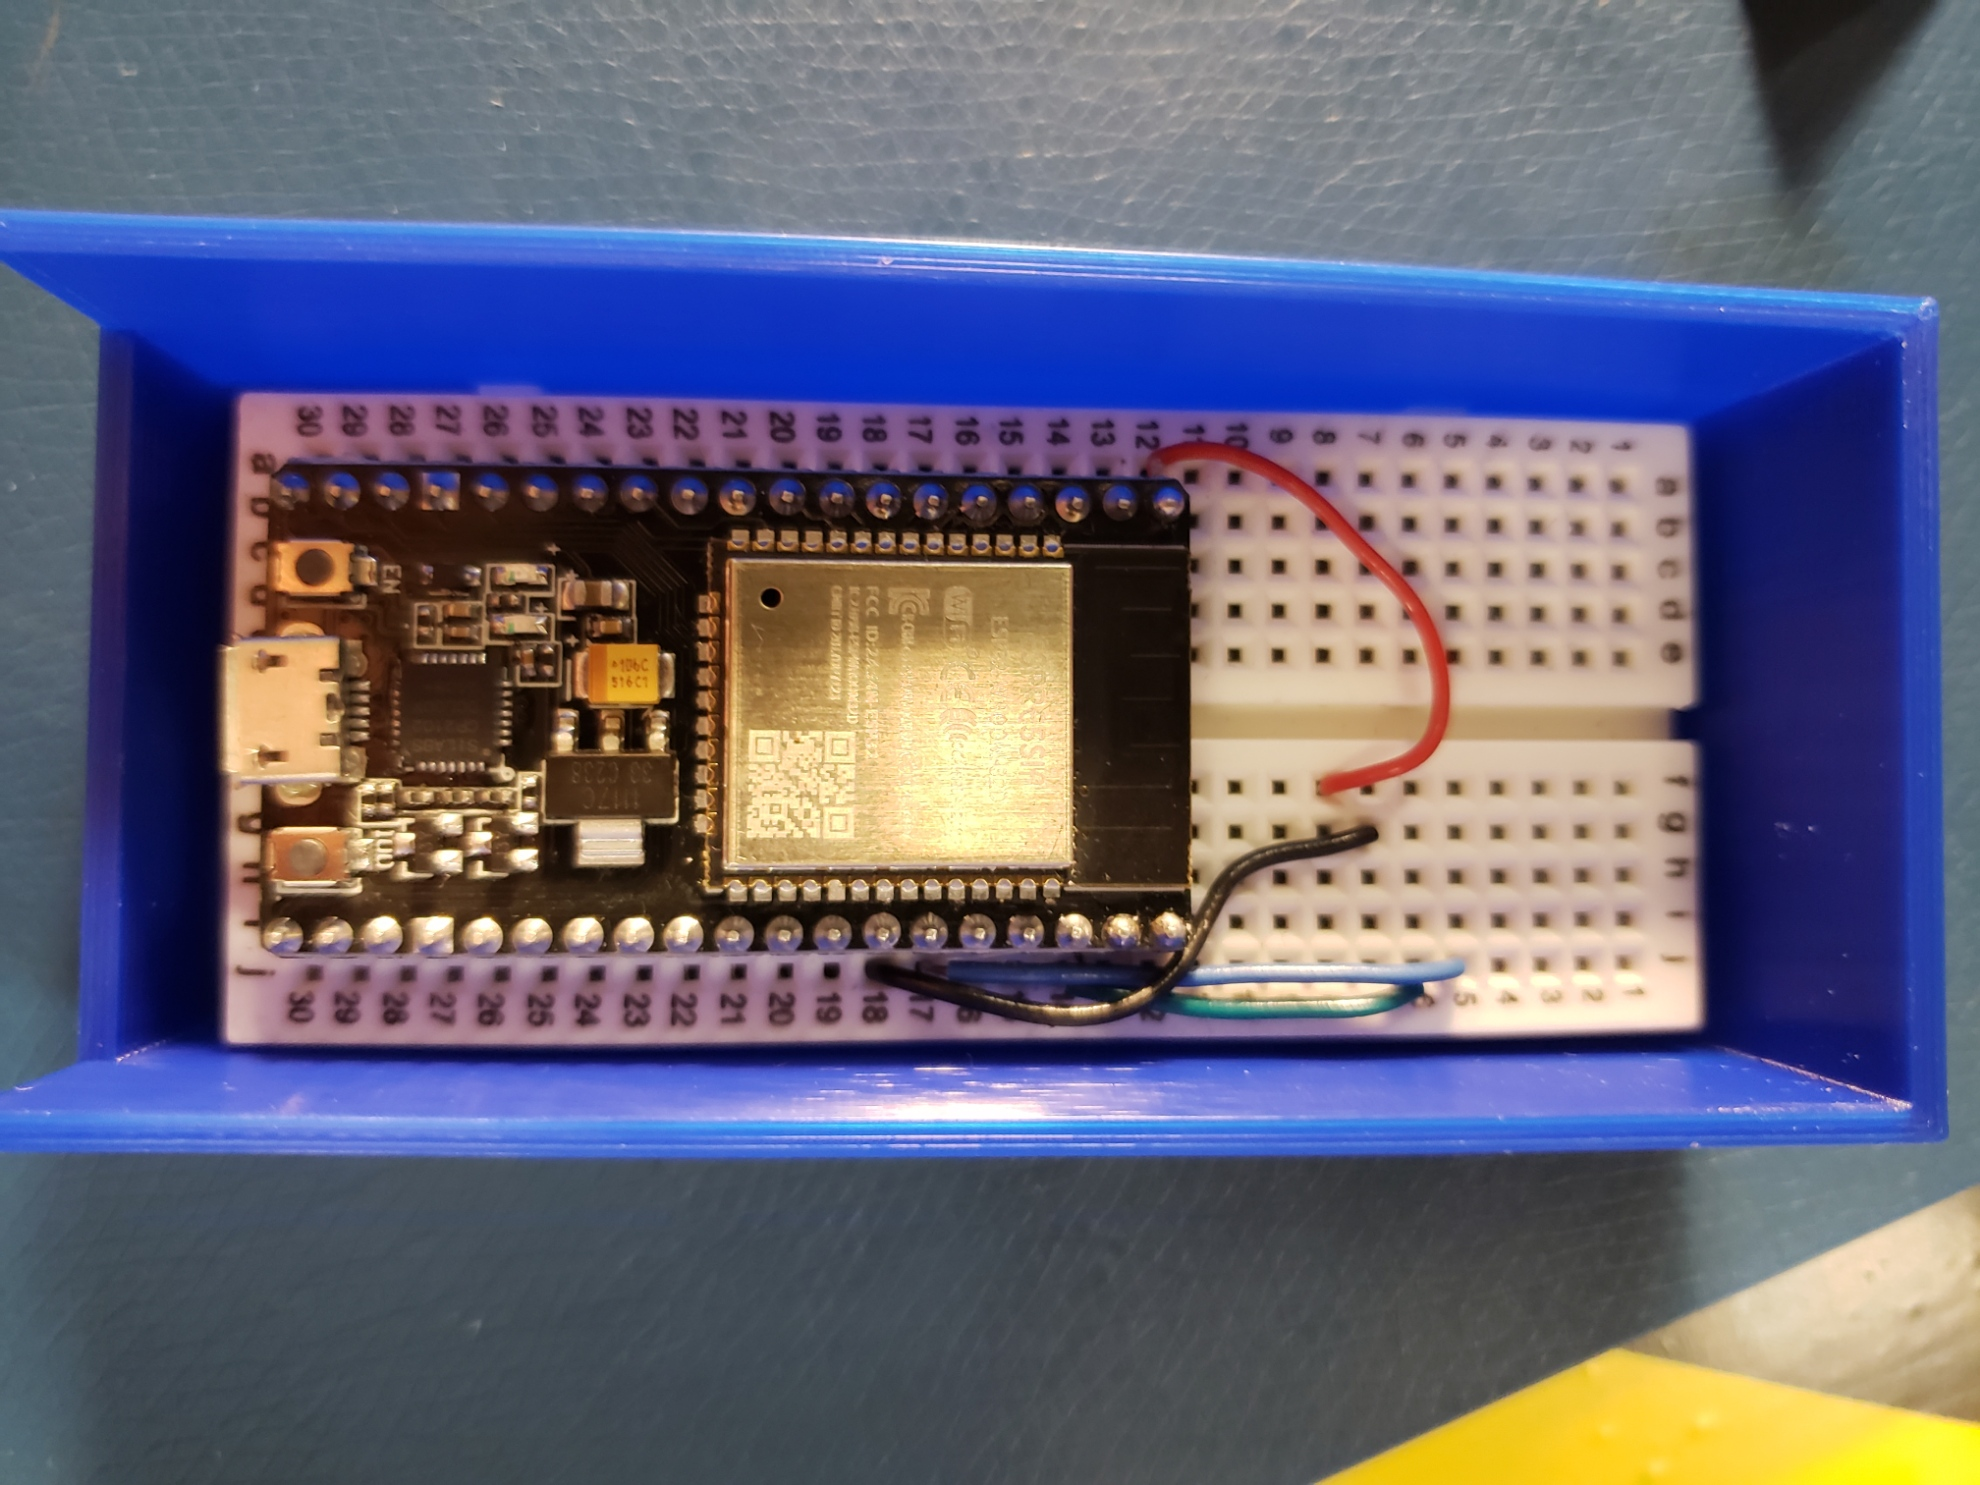
\includegraphics[width=0.5\textwidth]{bb_wiring}
    \caption{Wiring of the breadboard.}
  \end{figure}
  
\item Insert the MPU6050 as shown below. \textit{VCC} should match up with the
  red wire. The breadboard is now completed.
  \begin{figure}[H]
    \centering
    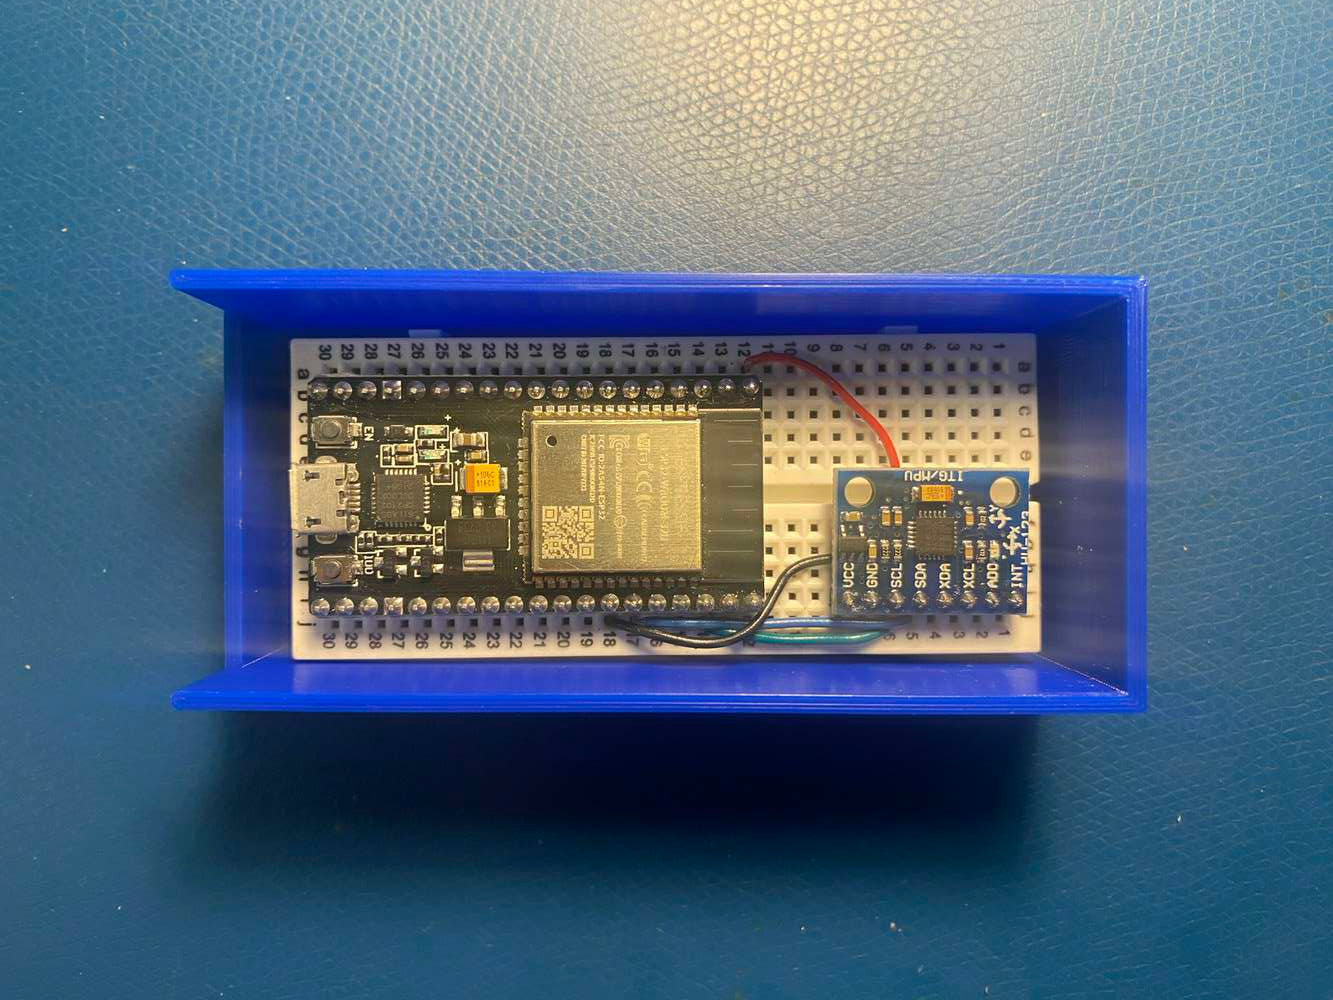
\includegraphics[width=0.5\textwidth]{bb_done2}
    \caption{The completed breadboard.}
  \end{figure}
  
\item Download the project code
  from
  \href{https://github.com/MrAwesomeRocks/dtc-head-tracker/archive/refs/heads/master.zip}{this
    link} and unzip the file.
  
\item Open the downloaded directory with VSCode. PlatformIO should now
  automatically load.
  
\item Once in VSCode, press the checkmark on the bottom left-hand corner of the
  screen to build the project.
  
\item Plug in the ESP32 to your computer. If on Windows, it will show up
  under \textit{Device Manager $\rightarrow$ Serial Devices}.\\
  \\
  \textit{Note: you may have to download a Serial driver. See your ESP32 vendor
    for details.}
  
\item Use the upload button (little arrow in bottom left) to upload the code to
  the ESP32.\\
  \\
  \textit{Note: you may have to put the ESP32 in bootloader mode first (hold
    the} \verb|IO0| \textit{button, press the} \verb|EN| \textit{button, and
    release} \verb|IO0| \textit{once uploading commences).}

\item Click the monitor button (the little plug) to check to make sure
  everything is working. There should be a line that looks like:\\
  \\
  \color{ForestGreen}\verb|[....][3][src/main.cpp] MPU6050 setup completed successfully!|
\end{enumerate}

\begin{figure}[h]
  \centering
  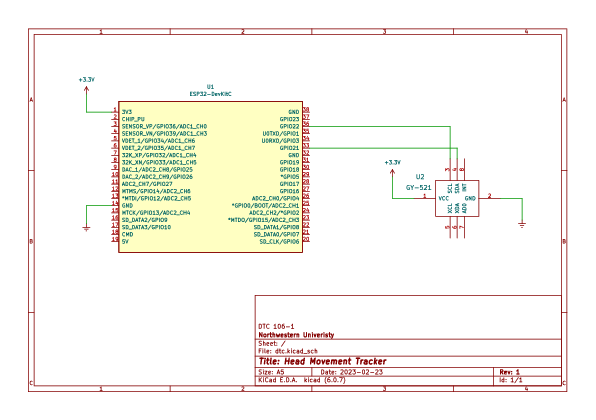
\includegraphics[width=\textwidth]{schematic}
  \caption{Wiring Schematic.}
  \label{fig:schematic}
\end{figure}


%%% Local Variables:
%%% mode: latex
%%% TeX-master: "../final_report"
%%% End:
